\chapter{Welcome to the Pit: Variables \& Data Types}

\begin{figure}[h!]
    \centering
    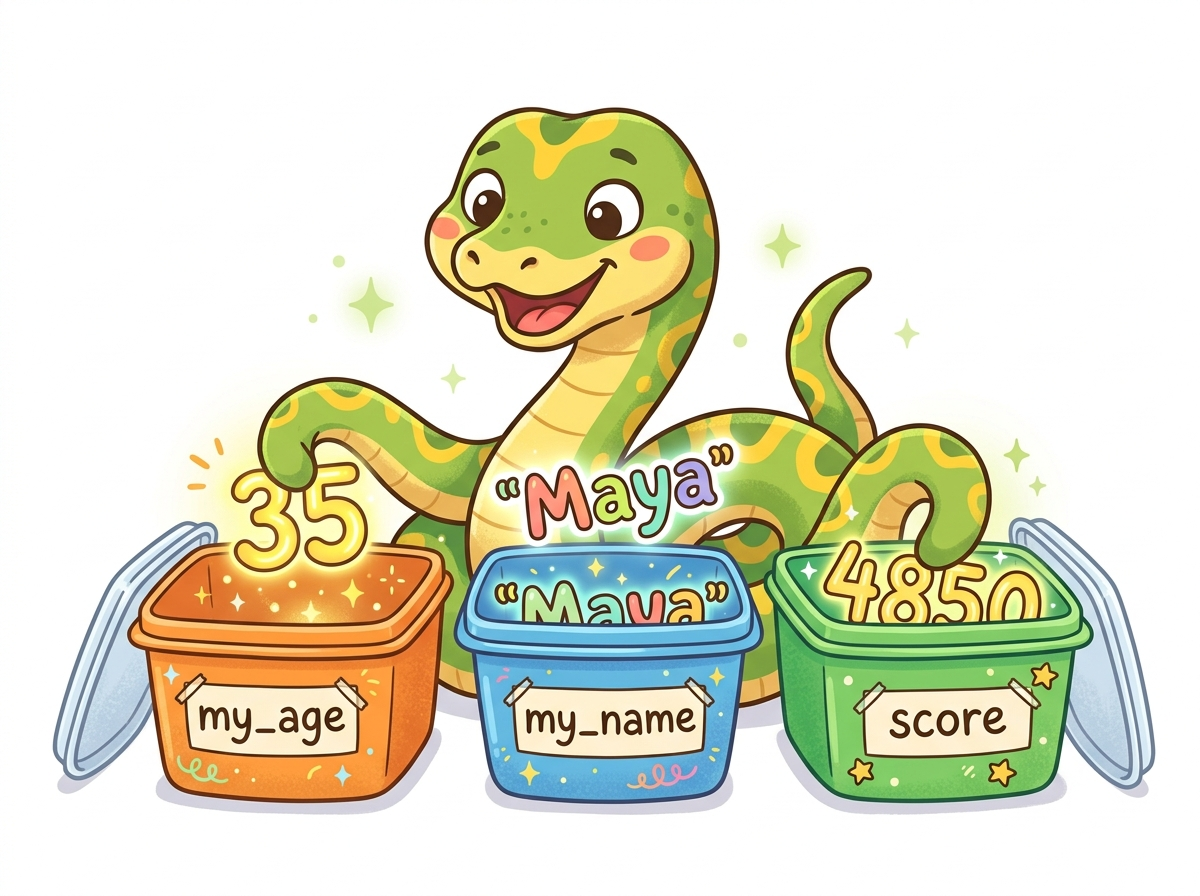
\includegraphics[width=0.75\textwidth]{images/ch1_tupperware.jpg}
    \caption{Variables in Python are like labeled Tupperware containers holding your valuable data.}
\end{figure}

\section{What is Code Anyway?}

Welcome, courageous snake charmer! Programming is simply the art of giving orders to a very fast, extremely loyal, but shockingly literal silicon rock called a CPU. If you tell a CPU to jump off a bridge, it won't ask ``Why?''; it will ask ``At what speed and angle in meters per second?''.

Python is one of the most friendly programming languages ever invented. Instead of cryptic binary numbers or terrifying C code with pointer arrows, Python reads almost like plain English with strict punctuation habits.

\section{Variables: Labeled Tupperware Containers}

Imagine your computer's Memory (RAM) as a giant kitchen filled with blank plastic Tupperware containers. A \textbf{variable} is just a friendly sticky note label you slap onto one of those containers so you can find your data later.

In Python, creating a variable is as simple as using the equals sign (\texttt{=}), which is called the \textbf{assignment operator}.

\begin{pycode}{Variables in Action}
# Slapping sticky notes on memory containers
my_age = 25
my_name = "Maya the Python"
is_hungry = True
coffee_cups = 3.5

# Displaying our loot to the world
print(my_name)
print("Coffee cups consumed today:", coffee_cups)
\end{pycode}

\begin{chucklebreak}{Why not store everything in your brain?}
Because human brains forget where they parked their car 10 minutes ago, whereas computer memory can store millions of numbers with 100\% precision until you pull the plug!
\end{chucklebreak}

\section{The Four Fundamental Data Types}

Python automatically figures out what kind of data you put inside your container. Here are the big four fundamental types:

\begin{enumerate}
    \item \textbf{Integer (\texttt{int}):} Whole numbers without decimals. E.g., \texttt{42}, \texttt{-7}, \texttt{1000}.
    \item \textbf{Float (\texttt{float}):} Floating-point decimal numbers. E.g., \texttt{3.14159}, \texttt{-0.001}.
    \item \textbf{String (\texttt{str}):} Text characters enclosed in quotes. E.g., \texttt{"Hello World!"}, \texttt{'Snakes rule'}.
    \item \textbf{Boolean (\texttt{bool}):} Absolute truth values. Only two exist: \texttt{True} or \texttt{False}.
\end{enumerate}

\begin{pycode}{Checking Data Types with type()}
x = 100
y = 3.14
z = "Python"
flag = True

print(type(x))     # <class 'int'>
print(type(y))     # <class 'float'>
print(type(z))     # <class 'str'>
print(type(flag))  # <class 'bool'>
\end{pycode}

\begin{viperpitfall}{Quotations Matter!}
Mixing up strings and numbers is a classic rookie mistake!
\texttt{x = 5} is a number you can do math with.
\texttt{x = "5"} is a piece of text! If you add \texttt{"5" + "5"}, Python won't give you \texttt{10} --- it will give you \texttt{"55"}!
\end{viperpitfall}

\section{Dynamic f-strings: Talking to Humans}

When you want to blend variables seamlessly into sentences, Python's \textbf{f-strings} (formatted string literals) are your best friend. Put an \texttt{f} right before the opening quote, and put variable names inside curly braces \texttt{\{\}}.

\begin{pycode}{f-String Magic}
name = "Cornelius"
pet = "Python"
age = 4

# Elegant f-string output
greeting = f"Hello, I am {name} the {pet}, and I am {age} years old!"
print(greeting)
\end{pycode}

\section{Code Example: The Wizard's Shopping Receipt}

Let's look at a practical example combining string input, type conversion, basic math, and f-strings to calculate a total potion bill.

\begin{pycode}{Shopping Receipt Calculator}
item_name = "Dragon Health Potion"
item_price = 15.50
quantity = 3
tax_rate = 0.08  # 8% tax

# Math calculations
subtotal = item_price * quantity
tax_amount = subtotal * tax_rate
grand_total = subtotal + tax_amount

# Printable receipt
print("--- WIZARD INN RECEIPT ---")
print(f"Item: {item_name} (x{quantity})")
print(f"Subtotal: ${subtotal:.2f}")
print(f"Tax (8%): ${tax_amount:.2f}")
print(f"Grand Total: ${grand_total:.2f}")
print("--------------------------")
\end{pycode}

\begin{snakesnack}{Variable Naming Rules}
Variable names in Python should be lowercase with words separated by underscores (called \texttt{snake\_case}). 
\begin{itemize}
    \item Good: \texttt{dragon\_health}, \texttt{user\_score\_2}
    \item Bad: \texttt{2nd\_user} (cannot start with a number!)
    \item Dangerous: \texttt{class}, \texttt{def}, \texttt{if} (these are reserved keywords!)
\end{itemize}
\end{snakesnack}

\section{Practice Problems \& Exercises}

Try solving these 3 practice problems to test your knowledge of variables and data types!

\begin{snakelab}{Problem 1.1: The Dragon's Loot Splitter (Easy)}
Write a script that divides $100$ gold coins equally among $3$ adventurer party members. 
\begin{itemize}
    \item Calculate how many coins each member gets using integer division (\texttt{//}).
    \item Calculate how many coins are left over for the dragon using the modulo operator (\texttt{\%}).
    \item Print the results using f-strings!
\end{itemize}
\end{snakelab}

\begin{pycode}{Solution 1.1: Dragon's Loot Splitter}
total_gold = 100
party_members = 3

coins_per_person = total_gold // party_members  # 33
leftover_gold = total_gold % party_members       # 1

print(f"Each adventurer receives {coins_per_person} gold coins.")
print(f"The greedy dragon keeps {leftover_gold} coin as tribute!")
\end{pycode}

\begin{snakelab}{Problem 1.2: Temperature Converter (Medium)}
Write a script that converts a temperature from Fahrenheit to Celsius using the formula:
\[ C = (F - 32) \times \frac{5}{9} \]
Test your program with $F = 98.6$ degrees and format the Celsius result to 1 decimal place.
\end{snakelab}

\begin{pycode}{Solution 1.2: Temperature Converter}
temp_f = 98.6
temp_c = (temp_f - 32) * (5 / 9)

print(f"{temp_f} degrees Fahrenheit is equal to {temp_c:.1f} degrees Celsius.")
\end{pycode}

\begin{snakelab}{Problem 1.3: Funny RPG Character Generator (Spicy)}
Write a script that stores a hero name, a weapon name, an agility level, and a luck score. 
Print out a comical character stats sheet with formatted lines and string repeating (e.g. \texttt{"=" * 30}).
\end{snakelab}

\begin{pycode}{Solution 1.3: RPG Character Generator}
hero_name = "Sir Reginald the Fluffy"
weapon = "Spoon of Doom"
agility = 12
luck = 99.5

banner = "=" * 32
print(banner)
print(f" HERO STATS: {hero_name.upper()}")
print(banner)
print(f" * Primary Weapon : {weapon}")
print(f" * Agility Score  : {agility}")
print(f" * Luck Rating    : {luck:.1f}%")
print(banner)
\end{pycode}
